\chapter{python Porosity Uptake Correlator (pyPUC)}
\label{ch:pyPUC}

\section{Introduction}

\section{Rationale for pyPUC}
\subsection{Dual isotherm analyses and relationship to low-pressure \ce{CO2} uptake}

\section{Software Design}

\newpage
\section[Publication III]{Publication III: Brute force determination of the optimum pore sizes for
\ce{CO2} uptake}

\textbf{Contribution of the author}: The author came up with the concept of the pyPUC software, designed and implemented it, and performed all analyses. A portion of the experimental work necessary to create DataSet 1, and all experimental work for DataSet 2 was also done by the author. The author wrote the paper in its entirety.

\newpage

\setlength{\originalVOffset}{\voffset}   
\setlength{\originalHOffset}{\hoffset}

\setlength{\voffset}{0cm}
\setlength{\hoffset}{0cm}
% too big for overleaf, try compilation later.
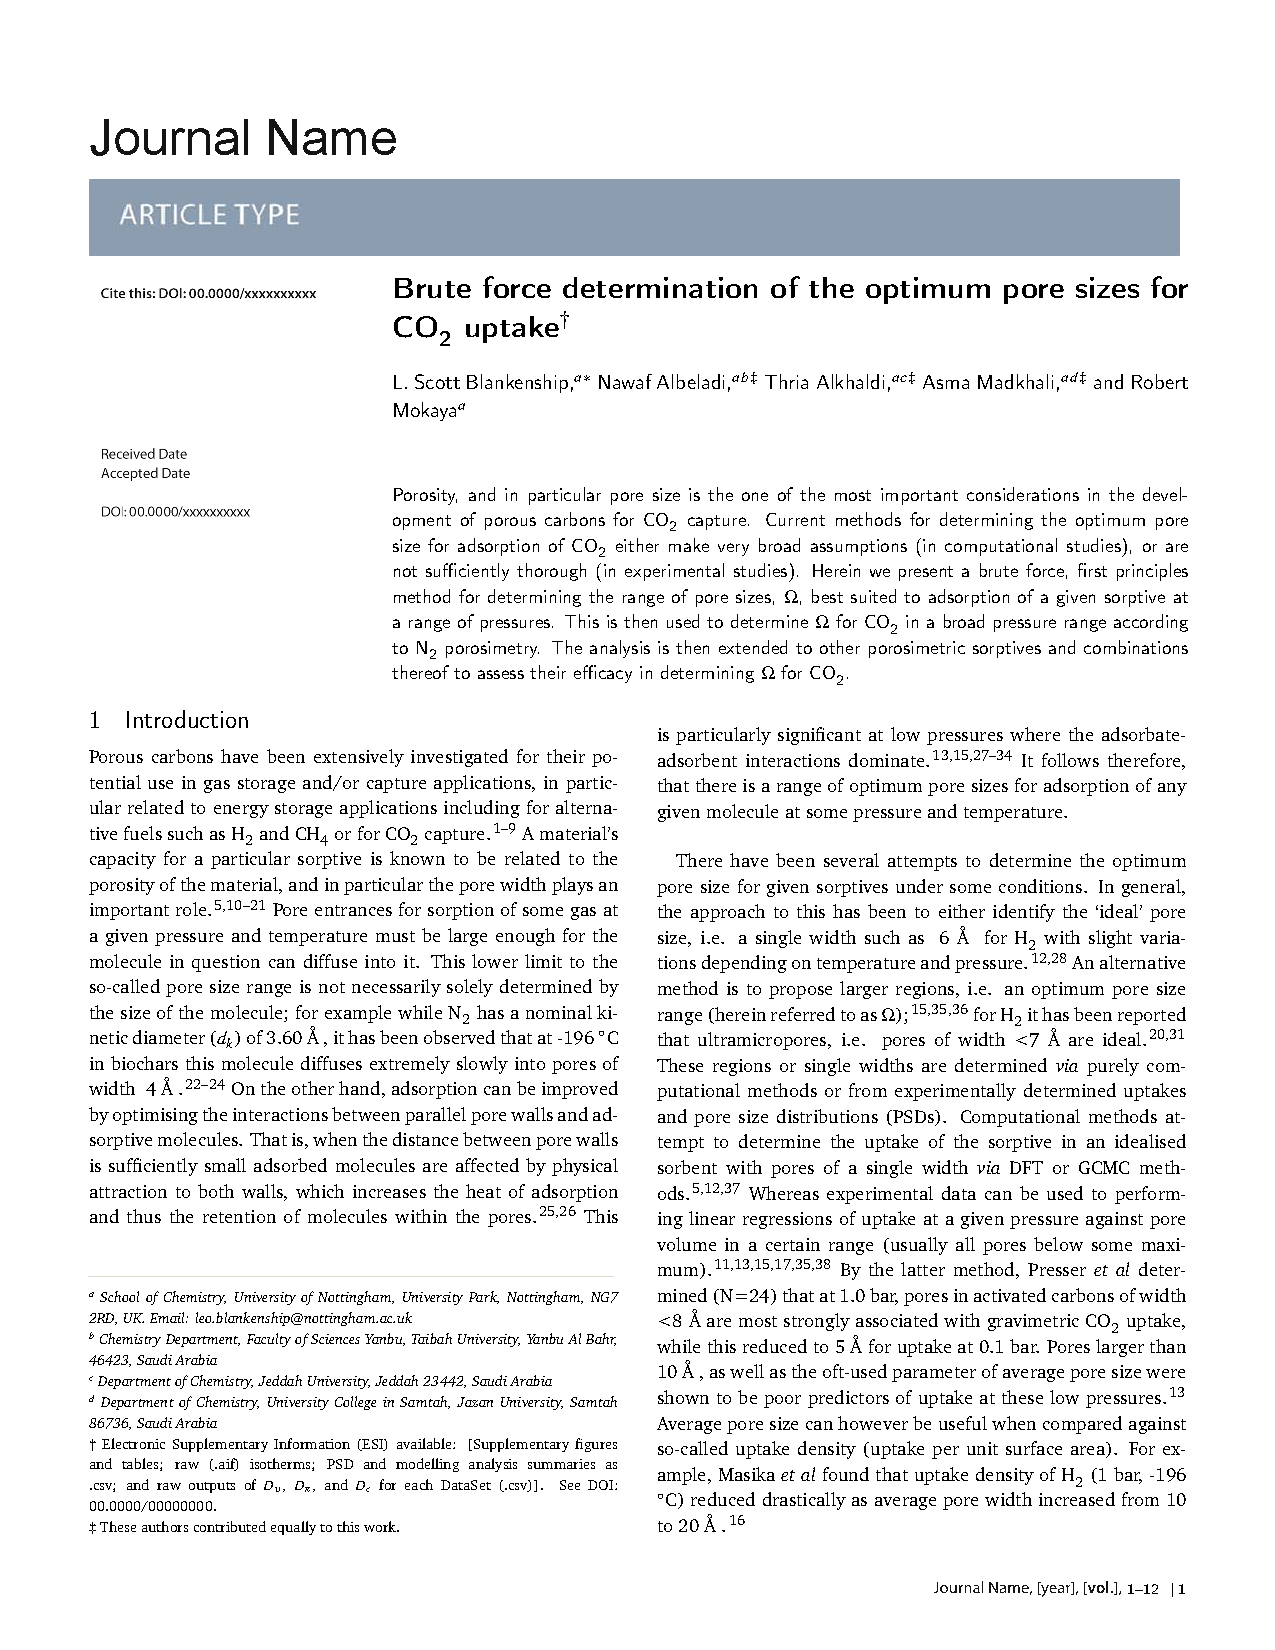
\includepdf[pages=-]{publication_03}
\setlength{\voffset}{\originalVOffset}
\setlength{\hoffset}{\originalHOffset}

\section{Summary \& Future Work}

\newpage
\section[Publication III Supporting Information]{Publication III Supporting Information: Brute force determination of the optimum pore sizes for \ce{CO2} uptake}

\newpage

\setlength{\originalVOffset}{\voffset}   
\setlength{\originalHOffset}{\hoffset}

\setlength{\voffset}{0cm}
\setlength{\hoffset}{0cm}
% too big for overleaf, try compilation later.
%\includepdf[pages=-]{si_03}
\setlength{\voffset}{\originalVOffset}
\setlength{\hoffset}{\originalHOffset}

\section*{References}